\newpage 
\chapter{Тема 17 Этапы загрузки ЭВМ}

\begin{center}{\bfseries Загрузка компьютера }
\end{center}
  
В кратком изложении загрузка компьютера происходит следующим образом. У каждого персонального компьютера есть материнская плата (которую теперь в США в результате распространения политкорректности на компьютерную индустрию называют родительской платой). На материнской плате находится программа, которая называется базовой системой ввода-вывода — BIOS (Basic Input Output System). BIOS содержит низкоуровневое программное обеспечение ввода-вывода, включая процедуры считывания состояния клавиатуры, вывода информации на экран и осуществления, ко всему прочему, дискового ввода-вывода. В наши дни эта программа хранится в энергонезависимой флеш-памяти с произвольным доступом, которая может быть обновлена операционной системой в случае обнаружения в BIOS различных ошибок. При начальной загрузке компьютера BIOS начинает работать первой. Сначала она проверяет объем установленной на компьютере оперативной памяти и наличие клавиатуры, а также установку и нормальную реакцию других основных устройств. Все начинается со сканирования шин PCIe и PCI с целью определения всех подключенных к ним устройств. Некоторые из этих устройств унаследованы из прошлого (то есть разработаны еще до создания технологии plug and play). Они имеют фиксированные уровни прерываний и адреса ввода-вывода (возможно, установленные с помощью переключателей или перемычек на карте ввода-вывода, но не подлежащие изменению со стороны операционной системы). Эти устройства регистрируются. Устройства, отвечающие стандарту plug and play, также регистрируются. Если присутствующие устройства отличаются от тех, которые были зарегистрированы в системе при ее последней загрузке, то производится конфигурирование новых устройств. Затем BIOS определяет устройство, с которого будет вестись загрузка, по очереди проверив устройства из списка, сохраненного в CMOS-памяти. Пользователь может внести в этот список изменения, войдя сразу после начальной загрузки в программу конфигурации BIOS. Обычно делается попытка загрузки с компакт-диска (иногда с флеш-накопителя USB), если, конечно, таковой присутствует в системе. В случае неудачи система загружается с жесткого диска. С загрузочного устройства в память считывается первый сектор, а затем выполняется записанная в нем программа. Обычно эта программа проверяет таблицу разделов, которая находится в конце загрузочного сектора, чтобы определить, какой из разделов имеет статус активного. Затем из этого раздела считывается вторичный загрузчик, который в свою очередь считывает из активного раздела и запускает операционную систему. После этого операционная система запрашивает BIOS, чтобы получить информацию о конфигурации компьютера. Она проверяет наличие драйвера для каждого устройства. Если драйвер отсутствует, операционная система просит установить компакт-диск с драйвером (поставляемый производителем устройства) или загружает драйвер из Интернета. Как только в ее распоряжении окажутся все драйверы устройств, операционная система загружает их в ядро. Затем она инициализирует свои таблицы, создает все необходимые ей фоновые процессы и запускает программу входа в систему или графический интерфейс пользователя.

\newpage 
\chapter{Тема 18 Мониторинг ресурсов}

Действие аппаратной составляющей часов ограничивается выдачей прерываний через
известные интервалы времени. Все остальное, касающееся времени, должно быть сделано программным обеспечением — драйвером часов. Конкретные обязанности драйвера
часов варьируются в зависимости от используемой операционной системы, но чаще
всего в них включается практически всё из следующего списка:

\begin{enumerate}
  \item Ведение показаний времени суток.
  \item Предотвращение работы процессов дольше позволенного.
  \item Ведение учета использования центрального процессора.
  \item Обработка системного вызова alarm, выданного процессами пользователей.
  \item Предоставление сторожевых программируемых таймеров для компонентов самой операционной системы.
  \item Ведение аналитического, мониторингового и статистического сбора информации.
\end{enumerate}

Осуществление главной функции часов — ведения показаний времени суток (которое
также называется фактическим временем) не представляет особых трудностей. Нужно,
как упоминалось ранее, всего лишь увеличивать значение счетчика с каждым тактом
системных часов. Единственное, за чем нужно следить, — за количеством битов в счетчике времени суток. Если используются часы с частотой 60 Гц, то 32-разрядный счетчик
будет переполняться каждые два года. Понятно, что система не сможет хранить фактическое время в виде числа тактов системных часов с 1 января 1970 года в 32 битах.
Эту проблему можно решить тремя способами.

Первый способ предусматривает использование 64-разрядного счетчика, хотя при этом усложняется его обслуживание,
которое в течение секунды должно проводиться многократно. 

Второй способ заключается в ведении значения времени суток не в тактах, а в секундах с использованием
вспомогательного счетчика для подсчета тактов, пока не наберется целая секунда. Поскольку 232 с — это более 136 лет, этот метод позволит системе работать до XXII века.

При третьем способе подсчет ведется в тактах, но делается он относительно времени
начальной загрузки системы, а не какого-то конкретного внешнего момента времени.

При считывании значения резервных часов или после ввода пользователем фактического времени время начальной загрузки системы вычисляется из текущего времени
суток и сохраняется в памяти в удобной для системы форме. Чуть позже, когда будет
запрошено время суток, сохраненное время суток добавляется к счетчику, чтобы получить текущее время.

Вторая функция часов заключается в предотвращении излишне продолжительной
работы процессов. При каждом запуске процесса планировщик запускает его счетчик
кванта времени в тактах системных часов. При каждом прерывании от часов драйвер
часов уменьшает значение счетчика кванта времени на единицу. Когда значение достигает нуля, драйвер часов вызывает планировщик для возобновления работы другого
процесса.

Третья функция часов — ведение учета использования центрального процессора.

Наиболее точно это можно сделать за счет запуска второго таймера, не имеющего от-
ношения к главному таймеру системы, при каждом запуске процесса. Когда процесс
останавливается, значение таймера может быть считано и по нему можно будет судить
о продолжительности работы процесса. Чтобы все работало должным образом, значение второго таймера должно быть сохранено при выдаче прерывания и после этого
восстановлено. 

Менее точным, но более простым является способ ведения учета, при котором указатель на запись в таблице процессов, относящуюся к текущему выполняемому процессу,
содержится в глобальной переменной. При каждом такте системных часов значение
поля в записи текущего процесса увеличивается на единицу. Таким образом, каждый
такт системных часов «отводится» тому процессу, который в этот момент выполняется.
Но при такой стратегии возникает небольшая проблема, которая заключается в том, что
если за время работы процесса возникает множество прерываний, ему все равно отводится полный такт системных часов, даже если он и не проделал никакой существенной
работы. Строгий учет использования времени центрального процессора в условиях прерываний его работы ведет к большим затратам ресурсов и применяется крайне редко. Если драйвер часов располагает достаточным количеством последних, то он может
выделить отдельные часы для каждого запроса. Но если их не хватает, он может
имитировать несколько виртуальных часов, используя лишь одни физические часы.
К примеру, он может вести таблицу, в которой содержится время выдачи сигнала для
всех поддерживаемых им не завершивших свою работу таймеров, а также переменную,
предоставляющую время срабатывания ближайшего таймера. При каждом обновлении
времени суток драйвер проверяет, не пора ли выдать очередной сигнал. Если уже пора,
в таблице ищется, куда его послать.

Если ожидается множество сигналов, то лучше будет сымитировать несколько часов,
выстроив в единую цепочку все невыполненные запросы на прерывание от таймера
и составив связанный список. Каждая запись списка сообщает, сколько
тактов системных часов следует ожидать за предыдущим тактом перед выдачей сигнала. В данном примере ожидаются сигналы через 4203, 4207, 4213, 4215 и 4216 тактов.
С каждым тактом значение переменной Следующий сигнал уменьшается на единицу. Когда оно становится равным нулю, выдается сигнал, соответствующий первому элементу списка, и затем этот элемент из списка удаляется. Затем переменной Следующий сигнал присваивается
значение того элемента, который оказывается в начале списка, в данном примере это
значение равно четырем.

Компоненты операционной системы также нуждаются в установке таймеров. Это
так называемые сторожевые таймеры, часто применяемые для обнаружения таких проблем, как зависания.

Механизм, используемый драйвером часов для обработки сторожевых таймеров, почти аналогичен обработке пользовательских сигналов. Единственное отличие состоит
в том, что когда время таймера истекает, вместо выдачи сигнала драйвер часов вызывает процедуру, предоставленную обратившейся программой, частью кода которой
она и является. Процедура обратившейся программы может делать все, что ей нужно,
даже выдавать прерывание, хотя применение прерываний внутри ядра зачастую просто
мешает его работе, а сигналов там не существует. Именно поэтому и предоставляется механизм сторожевых таймеров. Следует заметить, что этот механизм работает только
в том случае, когда драйвер часов и вызываемая процедура находятся в одном и том же
адресном пространстве.

Последним в нашем списке фигурирует сбор информации для профилирования
программ. Некоторые операционные системы предоставляют механизм, с помощью
которого пользовательская программа может иметь систему построения гистограмм относительно показаний своего счетчика команд, чтобы можно было увидеть, на что расходуется ее время. Если такое профилирование возможно, то с каждым тактом драйвер
проверяет, профилируется ли текущий процесс, и, если он профилируется, вычисляет
номер ячейки суммирования (диапазон адресов), соответствующей текущему счетчику
команд. Затем значение этой ячейки увеличивается на единицу. Этот механизм может
быть использован также для профилирования самой системы.

Большинство компьютеров оборудовано вторыми программируемыми часами, которые
могут быть настроены на выдачу таймерных прерываний с любыми необходимыми
программе характеристиками. По отношению к таймеру основной системы, чьи функции были рассмотрены ранее, этот таймер является дополнительным. Пока частота
прерываний невысока, использование этого дополнительного таймера в прикладных
целях не вызывает никаких проблем. Трудности возникают при возрастании частоты
прерываний таймера, используемого в прикладных целях, до очень высоких значений.

Для управления вводом-выводом используются, как правило, два способа: прерывания
и опросы. Прерывания обладают небольшим временем задержки, то есть они происходят сразу же вслед за событием, с небольшой задержкой или вовсе без нее. В то же
время при использовании современных центральных процессоров прерывания приводят к существенным издержкам в силу необходимости переключения контекста и их
влияния на конвейерную обработку, буфер TLB и кэш.Программные таймеры позволяют избежать прерываний. Вместо них, как только управление по каким-то причинам передается ядру, непосредственно перед возвращением в режим пользователя осуществляется проверка значения фактического времени,
чтобы увидеть, не истекло ли время программного таймера. Если его время истекло, осуществляется запланированное событие (например, передача пакета или проверка наличия входящего пакета), при этом нет надобности переходить в режим ядра, поскольку
система в нем и находится. После выполнения запланированной задачи программный
таймер перезапускается, чтобы снова быть задействованным. Нужно лишь скопировать
текущее значение часов в таймер и добавить к нему время истечения ожидания события.

Программные таймеры устанавливаются или сбрасываются с частотой передачи
управления ядру, осуществляемого по каким-то другим причинам. В число этих при-
чин входят:

\begin{enumerate}
  \item системные вызовы;
  \item отсутствие адресов в буфере TLB;
  \item ошибки отсутствия страниц;
  \item прерывания ввода-вывода;
  \item отсутствие загруженности центрального процессора.
\end{enumerate}

Чтобы определить, как часто происходят эти события, Арон и Дрюшель провели измерения при нескольких вариантах загрузки центральных процессоров, включая полностью загруженный веб-сервер, веб-сервер, имеющий фоновые задачи, ограниченные
по скорости вычислений, воспроизведение аудиопотока, получаемого из Интернета
в реальном масштабе времени, а также перекомпиляцию ядра UNIX. Средняя частота
вхождений в ядро изменялась от 2 до 18 мкс, при этом причиной около половины
этих вхождений были системные вызовы. Таким образом, в первом приближении задача задействования программного таймера каждые 10 мкс была вполне выполнимой,
хотя и со случающимися время от времени нарушениями крайних сроков. Нечастые
опоздания на 10 мкс намного предпочтительнее, чем использование прерываний,
« съедающих» 35 процентов времени центрального процессора.

\newpage 
\chapter{Тема 19 Трансляция программ}

\begin{opr}
  Система программирования – это комплекс средств, предназначенный для создания и эксплуатации программ на конкретном языке программирования на ЭВМ определенного типа.
\end{opr}

Текстовый редактор позволяет набрать текст программы на языке программирования. Для этой цели можно использовать любой редактор, но лучше пользоваться специализированным текстовым редактором, входящим в стандартную комплектацию системы программирования, в котором ключевые слова выделяются различными цветами и шрифтами.

Языки программирования высокого уровня являются машинно-независимыми и требуют использования соответствующих программ-переводчиков (трансляторов) для представления программы на языке машины, на которой она будет исполняться. Идеи трансляции (перекодирования) одних символов в другие легли в основу создания различных языков программирования с соответствующими трансляторами. Транслятор – это основа системы программирования. 

\begin{utv}
  Трансляторы бывают двух типов – компиляторы и интерпретаторы.
\end{utv}

Отличие компиляторов от интерпретаторов заключается в процедуре трансляции текста в машинный код. Компилятор преобразует весь текст программы в последовательный набор машинных команд, который в дальнейшем отправляется на выполнение. Интерпретатор же осуществляет трансляцию по принципу последовательного синхронного перевода. Каждая отдельная строка программного текста транслируется, а затем, после ее интерпретации, команды этой строки выполняются. При каждом запуске программы на выполнение вся процедура полностью повторяется.

\begin{utv}
  Достоинство интерпретатора – удобство отладки программы в интерактивном режиме, а недостаток – малая скорость работы.
\end{utv}

Современные трансляторы с языков программирования высокого уровня, систем управления базами данных интегрируют в себе возможности и достоинства компиляторов и интерпретаторов, а в системы программирования добавляют различные сервисные утилиты по трансляции и отладке создаваемых программ.

Важнейшим элементом в развитии систем программирования выступили подпрограммы.

Подпрограммы бывают двух видов: процедуры и функции. Первые просто выполняют последовательность операторов, а вторые вычисляют значение и передают его в главную программу.

\begin{opr}
  Подпрограмма-процедура или подпрограмма-функция – это отдельный блок операторов, начинающийся заголовком и заканчивающийся признаком конца процедуры или функции.
\end{opr}

Чтобы подпрограмма имела смысл, ей надо получить какие-то значения, называемые параметрами. Параметры, которые принимаются в подпрограмме, описываются в заголовке и называются формальными. Обращение из главной программы к процедуре осуществляется по имени этой подпрограммы-процедуры с перечнем в скобках параметров, которые ей передаются; эти передаваемые параметры называются фактическими. Итак, при выполнении процедуры или функции формальные параметры временно заменяются на фактические.

Появление аппарата подпрограмм существенно облегчило процесс разработки системных и прикладных программ за счет формирования библиотек из наиболее часто употребляемых в программах алгоритмов – процедур и функций. В системах программирования обязательно присутствуют стандартные (встроенные в систему) библиотеки подпрограмм (файлы с расширением .lib), например, подпрограммы вычисления математических функций.

В настоящее время распространены пользовательские и прикладные библиотеки подпрограмм; их число увеличивается; меняется структура библиотечных подпрограмм. В современных языках получили распространение модули (Unit), представляющие собой специализированные пакеты взаимосвязанных подпрограмм определенного назначения, например, по работе с клавиатурой, с графикой и пр. Развитие объектно-ориентированного программирования позволило создавать библиотеки объектов и подпрограмм с объектными типами данных (Object). Примером могут служить оболочки типа Turbo Vision в языках Pascal и C.

Современная программа представляет собой набор команд, операторов и выражений, в которых имеются ссылки (прямые или косвенные) на различные подпрограммы из существующих в системе программирования библиотек, модулей, объектов. В этой связи исходный текст программы, как правило, занимает по объему места в памяти в несколько раз меньше, чем его оттранслированный вариант в машинных кодах.

Текст программы по отношению к процессу трансляции выступает как исходный модуль. При выполнении программы прежде всего необходимо перевести его в машинный двоичный код, называемый абсолютным или загрузочным модулем. Для этого на первых этапах осуществляется трансляция исходного текста в машинный код (объектный модуль), который, однако, еще не может быть использован для выполнения программы. Объектный модуль (файл с расширением .obj) содержит текст программы на машинном языке и дополнительную информацию, обеспечивающую настройку модуля по месту его загрузки и его объединение с другими независимо оттранслированными модулями в единую программу.

Следующий шаг трансляции – компоновка – заключается в подключении к исходному объектному модулю объектных модулей соответствующих подпрограмм в места ссылок на них. После компоновки или, иначе, редактирования связей возникает абсолютный модуль (файл с расширением .exe), намного превышающий по объему размер исходного текста программы и являющийся исполняемым компьютером после его запуска. Этот файл имеет самостоятельное значение и может работать под управлением той (или аналогичной) ОС, в которой он создан.

Редактор связей (иначе компоновщик или сборщик) представляет собой системную обрабатывающую программу, редактирующую и объединяющую объектные модули, полученные в результате работы транслятора, в единые загрузочные, готовые к выполнению программные модули, загружающиеся ОС для выполнения в основную память.

Объектные модули не предназначены для непосредственного исполнения, поэтому в них обычно нет привязки составляющих их машинных команд к конкретному месту в ОЗУ. Адреса машинных слов бывают условными, что помогает компоновщику размещать объектные модули в свободных местах ОЗУ, заменяя условные адреса команд на конкретные.

Многие системы программирования дополнительно содержат промежуточные этапы трансляции. В этих системах на первом шаге предусмотрена трансляция исходного текста в макроассемблерный код, а уже затем – в объектный модуль. Это связано с тем, что многие подпрограммы удобнее писать на Ассемблере, и подключать их легче на этапе объединения (связывания) ассемблерного модуля с ассемблерными библиотеками подпрограмм.

В современные системы программирования входят отладчики, позволяющие анализировать работу программы по шагам и предоставляющие средства для просмотра и изменения значений переменных в ходе отладки программы, поиска ошибок и т.д. Использование отладчиков значительно облегчает процесс доводки больших программ.

Описанный процесс трансляции характерен для компиляции. Последовательно реализованный интерпретатор объектного модуля фактически не создает. В этом его недостаток, а достоинство – в экономии машинной памяти. Впрочем, у современных ЭВМ, в том числе и ПК, проблема малого ОЗУ отходит на второй план, и интерпретация встречается все реже, т.к. эффективность этого процесса в целом значительно ниже. К компилируемым языкам программирования можно отнести, например, Pascal, C, C++, а к интерпретируемым – Basic.

\begin{utv}
  Трансляция происходит в три этапа:
  \begin{enumerate}
    \item синтаксический анализ. Транслятор проверяет, не нарушены ли в исходной программе формальные правила, содержащиеся в данном языке программирования. В системе программирования встроены описания всех синтаксически разрешенных конструкций, и транслятор применяет их к исходной программе. Для строгого и точного задания синтаксиса применяются специальные метаязыки (языки для описания других языков) – нормальные металингвистические формы Бэкуса-Наура (язык БНФ) и синтаксические диаграммы Вирта. Первой фазой синтаксического анализа является лексический анализ, заключающийся в просмотре литер исходной программы и построении из них лексически допустимых единиц – идентификаторов, ключевых слов языка, чисел и т.д. Во второй фазе эти единицы уже рассматриваются как неделимые, и проверяется допустимость их сочетания;
    \item семантический анализ. Транслятор проверяет, имеет ли программа смысл в рамках данного языка программирования, т.е. понятен ли текст программы (семантика – смысловая сторона языка). Пример семантической ошибки – неописание переменных в языке, требующем обязательного явного их описания;
    \item собственно перевод операторов программы в машинный код. Однако и на этой стадии не исключены ошибки этапа исполнения (деление на ноль, выход за границу массива, переполнение разрядов и т.п.).
  \end{enumerate}
\end{utv}

Различные фазы компиляции могут быть как последовательными, так и частично перекрывающимися во времени. В зависимости от способа реализации компилятор читает и обрабатывает исходный текст один или несколько раз, называясь однопроходным, двухпроходным и т.д.

В интегрированной системе программирования все этапы создания программы автоматизированы; после того, как исходный текст программы введен, его компиляция и сборка осуществляются буквально одним нажатием клавиши.

\begin{center}{\bfseries СВОЙСТВА АЛГОРИТМОВ}
\end{center}

\begin{enumerate}
  \item точность – алгоритм должен однозначно и подробно описывать задачу;
  \item дискретность (упорядоченность) – все действия в алгоритме должны быть выстроены в четком, строго определенном порядке;
  \item результативность (эффективность) – алгоритм должен быть как можно более компактным, то есть результат должен быть получен при использовании минимально возможного числа программных шагов;
  \item массовость – алгоритм должен быть как можно более универсальным, подходящим для решения различных типов задач.
\end{enumerate}

\begin{center}{\bfseries Структура современных систем программирования }
\end{center}

\begin{figure}
  \begin{center}
  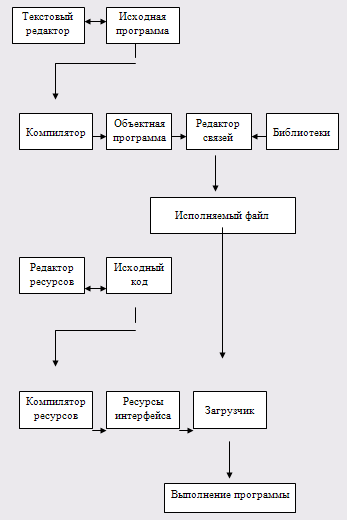
\includegraphics[width=250]{pic19-1}
  \end{center}
  \end{figure}

  \begin{opr}
    Система программирования - это комплекс программных средств, предназначенных для кодирования, тестирования и отладки программного обеспечения. Нередко системы программирования взаимосвязаны и с другими техническими средствами, служащими целям создания программного обеспечения на более ранних этапах жизненного цикла (от формулировки требований и анализа до проектирования).
  \end{opr}

  Системы программирования в современном мире доминируют на рынке средств разработки. Практически все фирмы-разработчики компиляторов поставляют свои продукты в составе соответствующей системы программирования в комплексе всех прочих технических средств. 

  Отдельные компиляторы являются редкостью и, как правило, служат только узкоспециализированным целям.

  Тенденция такова, что все развитие систем программирования идет в направлении неуклонного повышения их дружественности и сервисных возможностей. Это связано с тем, что на рынке в первую очередь лидируют те системы программирования, которые позволяют существенно снизить трудозатраты, необходимые для создания программного обеспечения на этапах жизненного цикла, связанных с кодированием, тестированием и отладкой программ. Показатель снижения трудозатрат в настоящее время считается более существенным, чем показатели, определяющие эффективность результирующей программы, построенной с помощью системы программирования.

  В качестве основных тенденций в развитии современных систем программирования следует указать внедрение в них средств разработки на основе так называемых "языков четвертого поколения" -- 4GL (four generation languages), -- а также поддержка систем "быстрой разработки программного обеспечения" -- RAD (rapid application development).

  Описание программы, построенное на основе языков 4GL, транслируется затем в исходный текст и файл описания ресурсов интерфейса, представляющие собой обычный текст на соответствующем входном языке высокого уровня. С этим текстом уже может работать профессиональный программист-разработчик -- он может корректировать и дополнять его необходимыми функциями. Такой подход позволяет разделить работу проектировщика, ответственного за общую концепцию всего проекта создаваемой системы, дизайнера, отвечающего за внешний вид интерфейса пользователя, и профессионального программиста, отвечающего непосредственно за создание исходного кода создаваемого программного обеспечения.

  В целом языки четвертого поколения решают уже более широкий класс задач, чем традиционные системы программирования. Они составляют часть средств автоматизированного проектирования и разработки программного обеспечения, поддерживающих все этапы жизненного цикла -- CASE-систем.

  \newpage 
\chapter{Тема 20 Формальные грамматики}

\begin{center}{\bfseries Алфавиты}
\end{center}

\begin{opr}
  Алфавитом называют конечное непустое множество символов.
\end{opr}

Условимся обозначать алфавиты символом $\sum$ . Наиболее часто используются следующие алфавиты:

\begin{enumerate}
  \item $\sum = (0,1)$ – бинарный алфавит.
  \item $\sum = (a,b, …,z)$ – множество строчных букв английского алфавита.
  \item Множество ASCII-символов или множество всех печатных ASCII- символов.
\end{enumerate}

\begin{center}{\bfseries Цепочки}
\end{center}

\begin{opr}
  Цепочка, или иногда слово, - это конечная последовательность символов некоторого алфавита. Например, 01101 – это цепочка в бинарном алфавите $\sum$ = (0,1). Цепочка 111 также является цепочкой в этом алфавите.  
\end{opr}

\begin{center}{\bfseries Пустая цепочка}
\end{center}

\begin{opr}
  Пустая цепочка – это цепочка, не содержащая ни одного символа. Эту цепочку, обозначаемую  $\epsilon$, можно рассматривать как  цепочку в любом алфавите.  
\end{opr}

\begin{center}{\bfseries Длина цепочки}
\end{center}

Часто оказывается удобным классифицировать цепочки по их длине, т.е по числу позиций для символов в цепочке. Например, цепочка 01101 имеет длину 5. Обычно говорят, что длина цепочки – это “число символов” в ней. Это определение широко распространено, но не вполне корректно. Так в цепочке 01101 всего 2 символа, но число позиций в ней – пять, поэтому имеет длину 5. Все же следует иметь в виду, что часто пишут “число символов”, имея в виду “число позиций”.

Длину некоторой цепочки w обычно обозначают |w|. Например, |011| = 3, a |$\epsilon$| = 0.

\begin{center}{\bfseries Степени алфавита}
\end{center}

Если $\sum$ – некоторый алфавит, то можно выразить множество всех цепочек определенной длины, состоящих из символов данного алфавита, используя знак степени. Определим $\sum^{k} $ как множество всех цепочек длины k, состоящих из символов алфавита $\sum$. 

\begin{example}
  Заметим, что $\sum0= ($\epsilon$)$ независимо от алфавита $\sum$, т.е $\epsilon$ – единственная цепочка длинны 0. 
\end{example}

Если $\sum$ = (0, 1), то $\sum^{1}$= (0, 1), $\sum^{2}$ = (00, 01, 10, 11), $\sum^{3}$ = (000, 001, 010, 011, 100, 101, 110, 111) и так далее. Отметим, что между $\sum$ и $\sum^{1}$ есть небольшое различие. Дело в том, что $\sum$ есть алфавит, и его элементы 0 и 1, каждая длинной 1. Мы не будем вводить разные обозначения для этих множеств, полагая, что их контекста будет понятно, является (0,1) или подобие ему множество алфавитом или же множеством цепочек. Множество всех цепочек над алфавитом $\sum$ принято обозначать $\sum^{*}$ . Так, например, (0,1)*= ($\epsilon$, 0, 1, 00, 01, 10, 11, 000, ...). По-другому это множество можно записать в виде $\sum^{*}$= $\sum^{0}$ U $\sum^{1}$ U $\sum^{2}$…

Иногда нам будет необходимо исключать из множества цепочек пустую цепочку. Множество всех непустых цепочек в алфавите $\sum$ обозначают через $\sum^{+}$. Таким образом, имеют место следующие равенства: 

$\sum^{+}$ = $\sum^{1}$ U $\sum^{2}$ U $\sum^{3}$\dots ;  $\sum^{*}$ = $\sum^{+}$ U $\sum^(\epsilon)$

\begin{center}{\bfseries Понятие языка. Способы задания языков}
\end{center}

\begin{opr}
  В общем случае язык - это заданный набор символов и правил, устанавливающих способы комбинации этих символов между собой для записи осмысленных текстов. Основой любого языка является алфавит, определяющий набор допустимых символов.
\end{opr}
 
Цепочка символов является цепочкой над алфавитом У: (У), если в нее входят только символы этого алфавита.

Если - некоторый алфавит, то:

+ - множество всех цепочек над алфавитом без .

* - множество всех цепочек над алфавитом , включая .

\begin{opr}
  Языком L над алфавитом У: L(У) - называют некоторое счетное подмножество цепочек конечной длины из множества всех цепочек над этим алфавитом. Множество цепочек языка не обязано быть конечным и каждая цепочка может иметь сколь угодно большую длину.
\end{opr}

Для любого языка L(У) справедливо L(У) У*.

Язык L(У) включает в себя язык L(У): L(У) L(У), если L(У) L(У).

Два языка совпадают (эквивалентны): L(У) = L(У), если L(У) L(У) и L(У) L(У).

Конкатенацией (объединением) языков L1 и L2 называют язык L, состоящий из всевозможных сцеплений цепочек языков L1 и L2: L = L1·L2 = (x·y | x L1, y L2).

Замыкание Клини, или итерация языка L, обозначается L* и определяется рекурсивно: 1) L0 = {л}, 2) Ln = L·Ln-1 для n > 0, 3) L* = Ln для всех n 0.

L+ = L*(л).

Язык L обладает суффиксным (префиксным) свойством, если никакая цепочка языка не является суффиксом (префиксом) другой цепочки.

Язык состоит из бесконечного множества цепочек символов над некоторым алфавитом, или слов. Но не любая цепочка символов над этим алфавитом принадлежит языку, т.к. существуют правила построения допустимых цепочек для каждого конкретного языка. Указать эти правила - значит задать язык. 

Существуют три основных способа задания языка:

\begin{enumerate}
  \item Перечисление всех допустимых цепочек языка (способ формальный, на практике нереализуем, т.к. в общем случае множество цепочек языка бесконечно и перечислить их невозможно).
  \item Указание способа порождения цепочек языка (задание грамматики языка) - применение т.н. генератора.
  \item Задание метода распознавания цепочек языка - использование распознавателя.
\end{enumerate}

Генераторы и распознаватели являются основными инструментами задания бесконечного языка конечными средствами. Существует определенная классификация языков по их типу, и для каждого класса языков имеются эквивалентные способы задания с помощью генераторов и распознавателей. Ниже рассмотрим эти способы более подробно.

В любом языке можно выделить его синтаксис и семантику. Кроме того, трансляторы имеют дело также с лексическими конструкциями (лексемами), которые задаются лексикой языка. Дадим определения этих понятий.

\begin{opr}
  Синтаксис языка - это набор правил, определяющий допустимые конструкции языка. Чаще всего синтаксис языка можно задать в виде строгого набора правил, но полностью это справедливо только для формальных языков.
\end{opr}

\begin{opr}
  Семантика языка - это раздел, определяющий значение предложений языка. Семантика определяет «содержание языка», т.е. задает значение всех допустимых цепочек языка. Для большинства языков семантика определяется неформальными методами.
\end{opr}

Лексика - это словарный запас языка. Лексическая единица (лексема) - конструкция, которая состоит из элементов алфавита языка и не содержит в себе других конструкций. Т.е. лексема может содержать в себе только элементарные символы алфавита и не может содержать других лексем. Например, лексемами русского языка являются слова, а пробелы и знаки препинания представляют собой разделители. Лексемами алгебры являются числа, знаки математических операций, обозначения функций и т.п. В языках программирования лексемы - это ключевые слова, идентификаторы, константы, метки, знаки операций.

\begin{center}{\bfseries Форма Бэкуса — Наура}
\end{center}

\begin{utv}
  Backus–Naur form или Backus normal form (BNF) это формальная система описания синтаксиса, в которой одни синтаксические категории последовательно определяются через другие категории. БНФ используется для описания контекстно-свободных формальных грамматик, обычно используется для описания синтаксиса языков программирования, форматов документов, наборов инструкций и протоколов связи. Применяются везде, где необходимо точное описание синтаксиса: например, в официальных спецификациях, руководствах и учебниках.
\end{utv}

Так же существует ещё и расширенная форма Бэкуса — Наура, отличающаяся более ёмкими конструкциями.

\begin{figure}[h]
  \begin{center}
  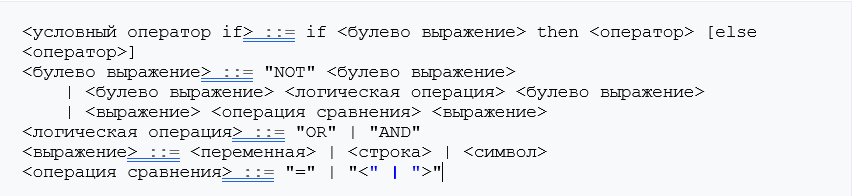
\includegraphics[width=450]{pic20-1}
  \end{center}
  \end{figure}

  \begin{center}{\bfseries Распознаватели}
  \end{center}
  
  Распознаватели классифицируют в зависимости от вида составляющих их компонентов: считывающего устройства, устройства управления и внешней памяти.

  По видам считывающего устройства распознаватели могут быть двусторонними и односторонними. Односторонние распознаватели допускают перемещение считывающей головки по ленте только в одном направлении, обычно слева направо (такой распознаватель называется левосторонним). Такие распознаватели не возвращаются назад к уже прочитанной части цепочки. Двусторонние распознаватели допускают перемещение считывающей головки в любом направлении.

  По видам устройства управления распознаватели бывают детерминированные и недетерминированные. Распознаватель является детерминированным, если для любой допустимой конфигурации существует не более одной следующей конфигурации. Если для любой допустимой конфигурации единственно возможна ровно одна следующая конфигурация, то такой распознаватель является детерминированным полностью определенным, иначе он неполностью определенный. Для недетерминированного распознавателя на некотором шаге возможно совершить несколько альтернативных переходов в различные конфигурации. При этом может оказаться, что только одна из возможных последовательностей шагов приводит в заключительную конфигурацию.

  По видам внешней памяти распознаватели бывают следующих типов:

  \begin{enumerate}
    \item Распознаватели без внешней памяти;
    \item Распознаватели с ограниченной внешней памятью;
    \item С неограниченной внешней памятью.
    \item Распознаватели без внешней памяти моделируются конечными автоматами и используют в процессе работы только конечную память УУ.
  \end{enumerate}

  Размер внешней памяти распознавателей второго типа ограничен. Эти ограничения могут носить характер некоторой функциональной зависимости от длины исходной цепочки символов - линейной, полиномиальной, экспоненциальной и т.п. Кроме того, может быть указан способ организации внешней памяти - стек, очередь, список и т.п. Например, широко распространены распознаватели с памятью магазинного типа, которая организована по стековому принципу.

  В распознавателях последнего типа предполагается, что для их работы может потребоваться внешняя память неограниченного объема, вне зависимости от длины входной цепочки. У таких распознавателей используется память с произвольным методом доступа.

  \begin{center}{\bfseries Задача разбора}
  \end{center}

  \begin{utv}
    Грамматики и распознаватели - два независимых метода, которые реально могут быть использованы для определения языка. Однако при разработке компилятора для некоторого языка программирования возникает задача, которая требует связать между собой эти два метода.
  \end{utv}

  Разработчики компилятора имеют дело с конкретным языком программирования, т.е. грамматика языка уже известна. Задача разработчиков состоит в построении распознавателя данного языка, который явится основой синтаксического анализатора в компиляторе.

  Итак, задача разбора формулируется следующим образом: на основе имеющейся грамматики некоторого языка необходимо построить распознаватель для этого языка. Заданная грамматика и распознаватель должны быть эквивалентны, т.е. определять один и тот же язык.

  В общем виде эта задача может быть решена не для всех типов языков, хотя для КС и регулярных языков задача разбора разрешима и существуют некоторые формальные методы ее решения.

  Компилятор должен не просто дать ответ, принадлежит ли входная цепочка данному языку, но и определить ее смысл. Фактически работа распознавателя в составе компилятора заключается в построении дерева разбора, которое затем используется для генерации кода. Кроме того, если исходная цепочка не принадлежит к заданному языку, компилятор должен не просто установить факт ошибки, но и по возможности определить ее тип и местоположение.

\begin{center}{\bfseries Классификация грамматик по Хомски}
\end{center}

Формальные грамматики классифицируются по структуре их правил.Если все без исключения правила грамматики удовлетворяют определённой структуре, то её относят к заданному типу. Если хотя бы одно правило грамматики не удовлетворяет требованиям структуры, то она не попадает в заданный тип. Если правила грамматики соответствуют структуре нескольких типов, то она будет отнесена по классификации к самому простому из них. Пусть грамматика обозначена как G(VT,VN,P,S), V=VT U VN. В соответствии с иерархией Хомского выделяют 4 типа грамматик.

\begin{center}{\bfseries 1. Тип 0 – грамматики с фразовой структурой, или без ограничений}
\end{center}

На структуру их правил не накладывается никаких ограничений, т.е. правила имеют вид: $\alpha$ → $\beta$ , где $\alpha$ $\in$ V^{+} , $\beta$ $\in$ V* . Это самый общий тип грамматик. Грамматики, которые относятся только к этому и не могут быть отнесены ни к какому другому типу, являются самыми сложными.

\begin{center}{\bfseries 2. Тип 1 – Контекстно-зависимые (КЗ) и неукорачивающие грамматики}
\end{center}

К этому типу относятся два основных класса грамматик.

\begin{figure}[h]
  \begin{center}
  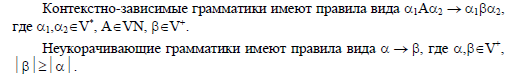
\includegraphics{pic20-2}
  \end{center}
\end{figure}

В КЗ-грамматиках при построении предложений заданного языка один и тот же нетерминальный символ может быть заменен различными терминальными цепочками в зависимости от контекста, в котором он встречается. Цепочки α1 и α2 в правилах обозначают контекст: α1 – левый контекст, α2 – правый контекст. В общем случае они могут быть пустыми. В неукорачивающих грамматиках при построении предложений языка цепочка символов заменяется на цепочку не меньшей длины. Эти два класса грамматик эквивалентны. При построении компиляторов такие грамматики не применяются, поскольку языки программирования имеют более простую структуру и могут быть построены с помощью грамматик других типов.

\begin{center}{\bfseries 3. Тип 2 – Контекстно-свободные (КС) грамматики}
\end{center}

V^{+}  $\alpha$ $\beta$ → $\in$ Контекстно-свободные (КС) грамматики имеют правила вида A → $\beta$ , где A $\in$ VN, $\beta$ $\in$ $V^{+}$ . В правой части у них стоит всегда хотя бы один символ. Их отличие от предыдущих типов состоит в том, что левая часть правил должна состоять ровно из одного нетерминального символа. Такие грамматики еще называют неукорачивающими контекстно-свободными (НКС) грамматиками. Существует почти эквивалентный им класс укорачивающих контекстно- свободных (УКС) грамматик, отличие которого в том, что он допускает пустую цепочку, т.е. правила имеют вид A → $\beta$, где A $\in$ VN, $\beta$ $\in$ V*. В дальнейшем, если возможность наличия в языке пустой цепочки не имеет принципиального значения, будем говорить просто о КС-грамматиках. КС-грамматики широко используются при описании синтаксических конструкций языков программирования.

  \begin{center}{\bfseries 4. Тип 3 – Регулярные грамматики}
  \end{center}

В правой части правил грамматик этого типа может присутствовать не более одного нетерминального символа, причём он должен быть расположен во всех правилах одной грамматики с одной и той же стороны от цепочки терминалов, а требования к левой части правил совпадают с предыдущим типом. К этому типу относятся два эквивалентных класса грамматик: леволинейные и праволинейные (их название определяется местоположением нетерминального символа в правой части правил относительно терминальной цепочки). Для любой праволинейной грамматики можно построить эквивалентную ей леволинейную, задающую тот же язык, и наоборот.

\begin{figure}[h]
    \begin{center}
    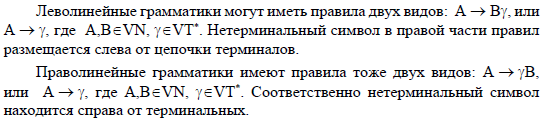
\includegraphics{pic20-3}
    \end{center}
\end{figure}

    Регулярные грамматики используются при описании простейших конструкций языков программирования: идентификаторов, констант, строк, комментариев и т.д. Они очень просты и удобны в использовании, поэтому в компиляторах на их основе строятся функции лексического анализа входного языка. Из определения типов видно, что любая регулярная грамматика является также КС-грамматикой, или любая грамматика может быть отнесена к типу 0. В то же время существуют УКС-грамматики, которые не относятся к типу 1, поскольку могут содержать правила вида A→λ, недопустимые в этом типе. В общем, сложность грамматики обратно пропорциональна тому максимально возможному номеру типа, к которому может быть отнесена эта грамматика. Самыми простыми являются грамматики типа 3, самыми сложными – типа 0.


    \begin{center}{\bfseries Классификация языков}
\end{center}

Существует множество классификаций языков программирования по различным критериям. Самое простое деление – на языки высокого и низкого уровня.

\begin{opr}
  Язык низкого уровня – это язык программирования, предназначенный для определенного типа компьютера и отражающий его внутренний машинный код; языки низкого уровня часто называют машинно-ориентированными языками. Их сложно конвертировать для использования на компьютерах с разными центральными процессорами, а также довольно сложно изучать, поскольку для этого требуется хорошо знать внутренние принципы работы компьютера.
\end{opr}

\begin{opr}
  Язык высокого уровня – это язык программирования, предназначенный для удовлетворения требований программиста; он не зависит от внутренних машинных кодов компьютера любого типа. Языки высокого уровня используют для решения проблем, и поэтому их часто называют проблемно-ориентированными языками. Каждая команда языка высокого уровня эквивалентна нескольким командам в машинных кодах, поэтому программы, написанные на языках высокого уровня, более компактны, чем аналогичные программы в машинных кодах.
\end{opr}

Другая классификация делит языки на вычислительные и языки символьной обработки.

Еще одна распространенная классификация языков программирования основана на принципе их организации, или парадигме. По этой классификации языки делят на процедурные (употребляются также термины императивные и структурные, хотя это не совсем одно и то же), объектно-ориентированные, функциональные и логические.

Функциональные и логические языки называют декларативными, или непроцедурными, поскольку программа представляет собой не набор команд, а описание действий, которые необходимо осуществить. Этот подход существенно проще и прозрачнее формализуется математическими средствами. Следовательно, программы проще проверять на наличие ошибок (тестировать), а также на соответствие заданной технической спецификации (верифицировать). Высокая степень абстракции также является преимуществом данного подхода. Фактически программист оперирует не набором инструкций, а абстрактными понятиями, которые могут быть достаточно обобщенными.

